\documentclass[a4paper,parskip,11pt, DIV12]{scrreprt}
\usepackage[english]{babel} % Für Deutsch [english] zu [ngerman] ändern. 
\usepackage[utf8]{inputenc}
\usepackage[T1]{fontenc}
\usepackage{lmodern}
\usepackage{blindtext}
\usepackage{graphicx}
\usepackage{caption}
\usepackage{subcaption}
%\renewcommand{\familydefault}{\sfdefault}
%\usepackage{helvet}
\usepackage{fancyhdr}
\usepackage{amsmath}
\usepackage{mdwlist} %Benötigt für Abstände in Aufzählungen zu löschen
\usepackage{framed} %Rahmen um Objekte
\usepackage{floatflt} %Text neben Bildern
\usepackage{colortbl} % Tabellen einfärben
\usepackage{here}
\usepackage{calc}
\usepackage{hhline}
\usepackage{marginnote}
\usepackage{chngcntr}
\usepackage{tabularx}
\usepackage{titlesec} % Textüberschriften anpassen

% \titleformat{Überschriftenklasse}[Absatzformatierung]{Textformatierung} {Nummerierung}{Abstand zwischen Nummerierung und Überschriftentext}{Code vor der Überschrift}[Code nach der Überschrift]

% \titlespacing{Überschriftenklasse}{Linker Einzug}{Platz oberhalb}{Platz unterhalb}[rechter Einzug]

\titleformat{\chapter}{\LARGE\bfseries}{\thechapter\quad}{0pt}{}
\titleformat{\section}{\Large\bfseries}{\thesection\quad}{0pt}{}
\titleformat{\subsection}{\large\bfseries}{\thesubsection\quad}{0pt}{}
\titleformat{\subsubsection}{\normalsize\bfseries}{\thesubsubsection\quad}{0pt}{}

\titlespacing{\chapter}{0pt}{-2em}{6pt}
\titlespacing{\section}{0pt}{6pt}{-0.2em}
\titlespacing{\subsection}{0pt}{5pt}{-0.4em}
\titlespacing{\subsubsection}{0pt}{-0.3em}{-1em}

%\usepackage[singlespacing]{setspace}
%\usepackage[onehalfspacing]{setspace}

\usepackage[
			%includemp,				%marginalien in Textkörper einbeziehen
			%includeall,
			%showframe,				%zeigt rahmen zum debuggen		
			marginparwidth=25mm, 	%breite der marginalien
			marginparsep=5mm,		%abstand marginalien - text
			reversemarginpar,		%marginalien links statt rechts
			%left=50mm,				%abstand von Seitenraendern
%			top=25mm,				%
%			bottom=50mm,
			]{geometry}		

%Bibliographie- Einstellungen
\usepackage[babel,german=quotes]{csquotes}
\usepackage[
   backend=bibtex8, 
   natbib=true,
    style=numeric,
    sorting=none
]{biblatex}
\bibliography{Quelle}
%Fertig Bibliographie- Einstellungen

\usepackage{hyperref}

\begin{document}

\begin{titlepage}
\begin{figure}[h]
\hfill

\includegraphics[scale=0.04]{uzh}
\end{figure}
\vspace{1 cm}
\textbf{\begin{huge}Labreport solid-state physics
\end{huge}}\\
\noindent\rule{\textwidth}{1.1 pt} \\

\begin{Large}\textbf{Resistivitymeasurement of a HTSC-Metal}
\end{Large}\\ 
\normalsize 
\par
\begingroup
\leftskip 0 cm
\rightskip\leftskip
\textbf{Modul:}\\ Solid state physics PHY210 \\ \\
\textbf{Assistance:}\\ Oleh Ivashko ; oleh.ivashko@physik.uzh.ch \\ \\
\textbf{Student:}\\ S.Hochrein, H.Imboden, S.Buse\\ \\
\textbf{Date:}\\ 13.06.2017 \\ \\
\par
\endgroup
\clearpage

\end{titlepage}


%Start Layout
\pagestyle{fancy}
\fancyhead{} 
\fancyhead[R]{\small \leftmark}
\fancyhead[C]{\textbf{Solid state physics} } 
\fancyhead[L]{
\includegraphics[height=2\baselineskip]{uzh}}

\fancyfoot{}
\fancyfoot[R]{\small \thepage}
\fancyfoot[L]{}
\fancyfoot[C]{}
\renewcommand{\footrulewidth}{0.4pt} 

\addtolength{\headheight}{2\baselineskip}
\addtolength{\headheight}{0.6pt}


\renewcommand{\headrulewidth}{0.6pt}
\renewcommand{\footrulewidth}{0.4pt}
\fancypagestyle{plain}{				% plain redefinieren, damit wirklich alle seiten im gleichen stil sind (ausser titlepage)
\pagestyle{fancy}}

\renewcommand{\chaptermark}[1]{ \markboth{#1}{} } %Das aktuelle Kapitel soll nicht Gross geschriben und Nummeriertwerden

\counterwithout{figure}{chapter}
\counterwithout{table}{chapter}
\counterwithout{equation}{chapter}
%Ende Layout

\tableofcontents





\chapter{Introduction}
Superconductivity in metals and alloys is characterized by a sudden disappearance of resistance for temperatures lower than a certain transition temperature, $T_c$. Not all materials can become superconducting and if they do, the temperature at which they do is not the same for different materials. Some only become superconducting at less than 5K (Mercury for example) while some can still be superconducting above 130K (Hg-Ba-Ca-Cu-O). \\
In our experiment, YBa$_2$Cu$_3$O$_{7-\mathrm{\delta}}$ was used. This material has a transition temperature of around 92K.

\begin{figure}[H]
\centering
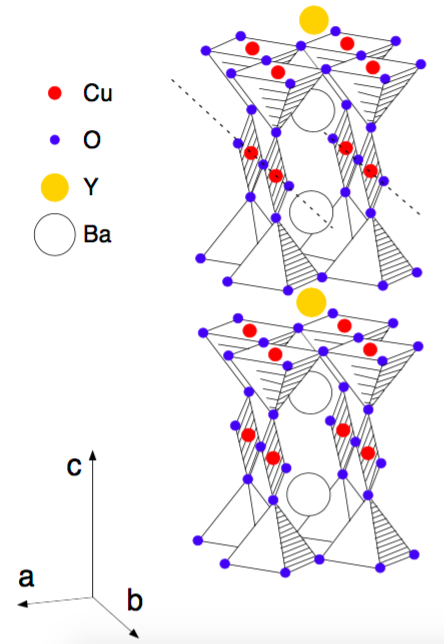
\includegraphics[width=6cm]{supercond.png}
\caption{Crystal structure of YBa$_2$Cu$_3$O$_{7-\mathrm{\delta}}$}
\end{figure}


\chapter{Experimental setup and Procedure}

The setup consists of four main parts \footnote{\url{http://www.physik.uzh.ch/data/peter/FestkoerperPhysik/InfoPraktFestkoerperphysik.shtml}}\\
\begin{itemize}
\item The specimen holder.\\
This is the container where the superconductor is placed. There are connections for the temperature sensor, the heating foil and for the resistance measurement.\\
\item The cryostat.\\
This part serves as a temperature regulator. The sample is enclosed in a tube, which is submerged in liquid nitrogen. To keep the sample at a certain temperature, a heating foil is attached behind the sample. This heating foil is needed, as liquid nitrogen has a constant temperature of around 77K at atmospheric pressure. \\
\item The vacuum system.\\
A vacuum of $2.8 \cdot 10^{-3}$mbar was created inside the tube. This vacuum helps to reduce the heat transfer between the probe and its surroundings, as heat is primarily exchanged through convection.\\ 
\item The electromagnet.\\
The tube with the sample is placed inside an electromagnet. Therefore the experiment can be repeated with different magnetic fields up to a field of 0.8T . 

\end{itemize}
\clearpage

\section*{Procedure}

The first step in the measuring process is the cooling. The sample and the apparatus are cooled by liquid nitrogen which gets pumped into the system. With the heating foil and the PID-controller an arbitrary temperature within the apparatus working range can be achieved. In the experiment the starting temperature was set to 82K. When this temperature was reached and stabilized the heating and cooling got turned off and the experiment started. While the samples temperature slowly increased due to the temperature difference to the room temperature, the resistance was measured. 
Since the sample is in a vacuum, the rise in temperature happens very slowly and we can assume the sample to be in thermal equilibrium. 

The resistivity measurement got realized in a four point measuring circuit. This setup is usually used when a resistance has to be measured precisely. 

\begin{figure}[H]
\centering
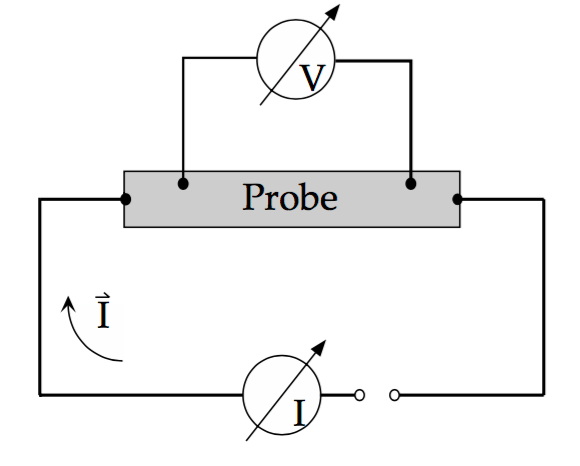
\includegraphics[width=6cm]{vierpunkt.png}
\caption{The four-point measuring technique}
\label{vierpunkt}
\end{figure}


Another measuring technique got used which at first glance may seem rather unusual. The direction of the current got reversed after each measurement. We can think of this as running the current in figure \ref{vierpunkt} first in clockwise direction and than in counterclockwise.


\chapter{Results}

\section{Questions}

\begin{enumerate}

\item Does YBa$_2$Cu$_3$O$_{7-\mathrm{\delta}}$  behave like a metal above the transition temperature? Describe the temperature dependence qualitatively.\\
\\
In the measured region just above the transition temperature, the resistance increases linearly with respect to the temperature. This corresponds to the expected behaviour of a metal. It can be seen in figure \ref{Res}.

\begin{figure}[H]
\centering
\includegraphics[scale=0.5]{Widerstand}
\caption[]{Measurement of the mean resistance.}
\label{Res}
\end{figure}
\hspace{0.1pt}

\item What is the expected dependence of the resistance of a metal (no superconductivity) due to an external magnetic field (for small magnetic fields)?\\
\\
For small magnetic fields, the resistance of a metal is independent due to an external magnetic field. The reason behind this is the Hall-effect. The magnetic field causes a Lorentz-force, acting on all moving electrons, perpendicular to the magnetic filed and the direction of the electrons velocity. Therefore the electrons concentrate on one side of the metal and an electric field, in the direction of the Lorentz-force appears. This causes a force on the electrons, in the opposite direction. As soon as the equilibrium is reached, where the two forces are equal, the electrons are able to move like if there was no magnetic field. Therefore, the resistance is the same. \\
This is not the case in the region near the transition temperature $T_c$ and below. It can also be seen in the measured data in figure \ref{Res}.

\hspace{0.1pt}

\item Determine the transition temperature, $T_c$. How do you do this?\\
\\
The transition temperature $T_c$ is defined as the temperature, at which the resistance of a superconducting material drops from a finite value to zero. In figure \ref{Res} one can see, that this is the point, where the slope of the resistance curve is maximal. Therefore, the derivative of the resistance curve was calculated numerically. Since the measured data has a lot of noise on top of the underling curve, the so called \emph{five-point-stencil method \footnote{\url{https://en.wikipedia.org/wiki/Five-point_stencil}}} was used to compute the derivative. Otherwise the peak would not be visible.

The \emph{five-point-stencil method} takes not only the next data points into account but also the 4 surrounding values. With this method we get a more smooth and useful curve. 

\begin{align*}
f'(x) \approx \frac{-f(x+2 h)+8 f(x+h)-8 f(x-h)+f(x-2h)}{12 h}
\end{align*}

In figure \ref{h1} the result of this method with $h = 1$ can be seen. This is still not good enough to find $T_c$. The five-point-stencil method with $h = 10$ gives a clearer indication to where the jump in resistance is located. This is due to the fact that by taking larger steps (making $h$ bigger), the noise has less impact. Even though successive measures oscillate quite a lot, the general behaviour of the measurements can be seen clearly in figure \ref{meanresist}. A larger step size will on average suppress the fluctuations.

\begin{figure}[H]
\centering
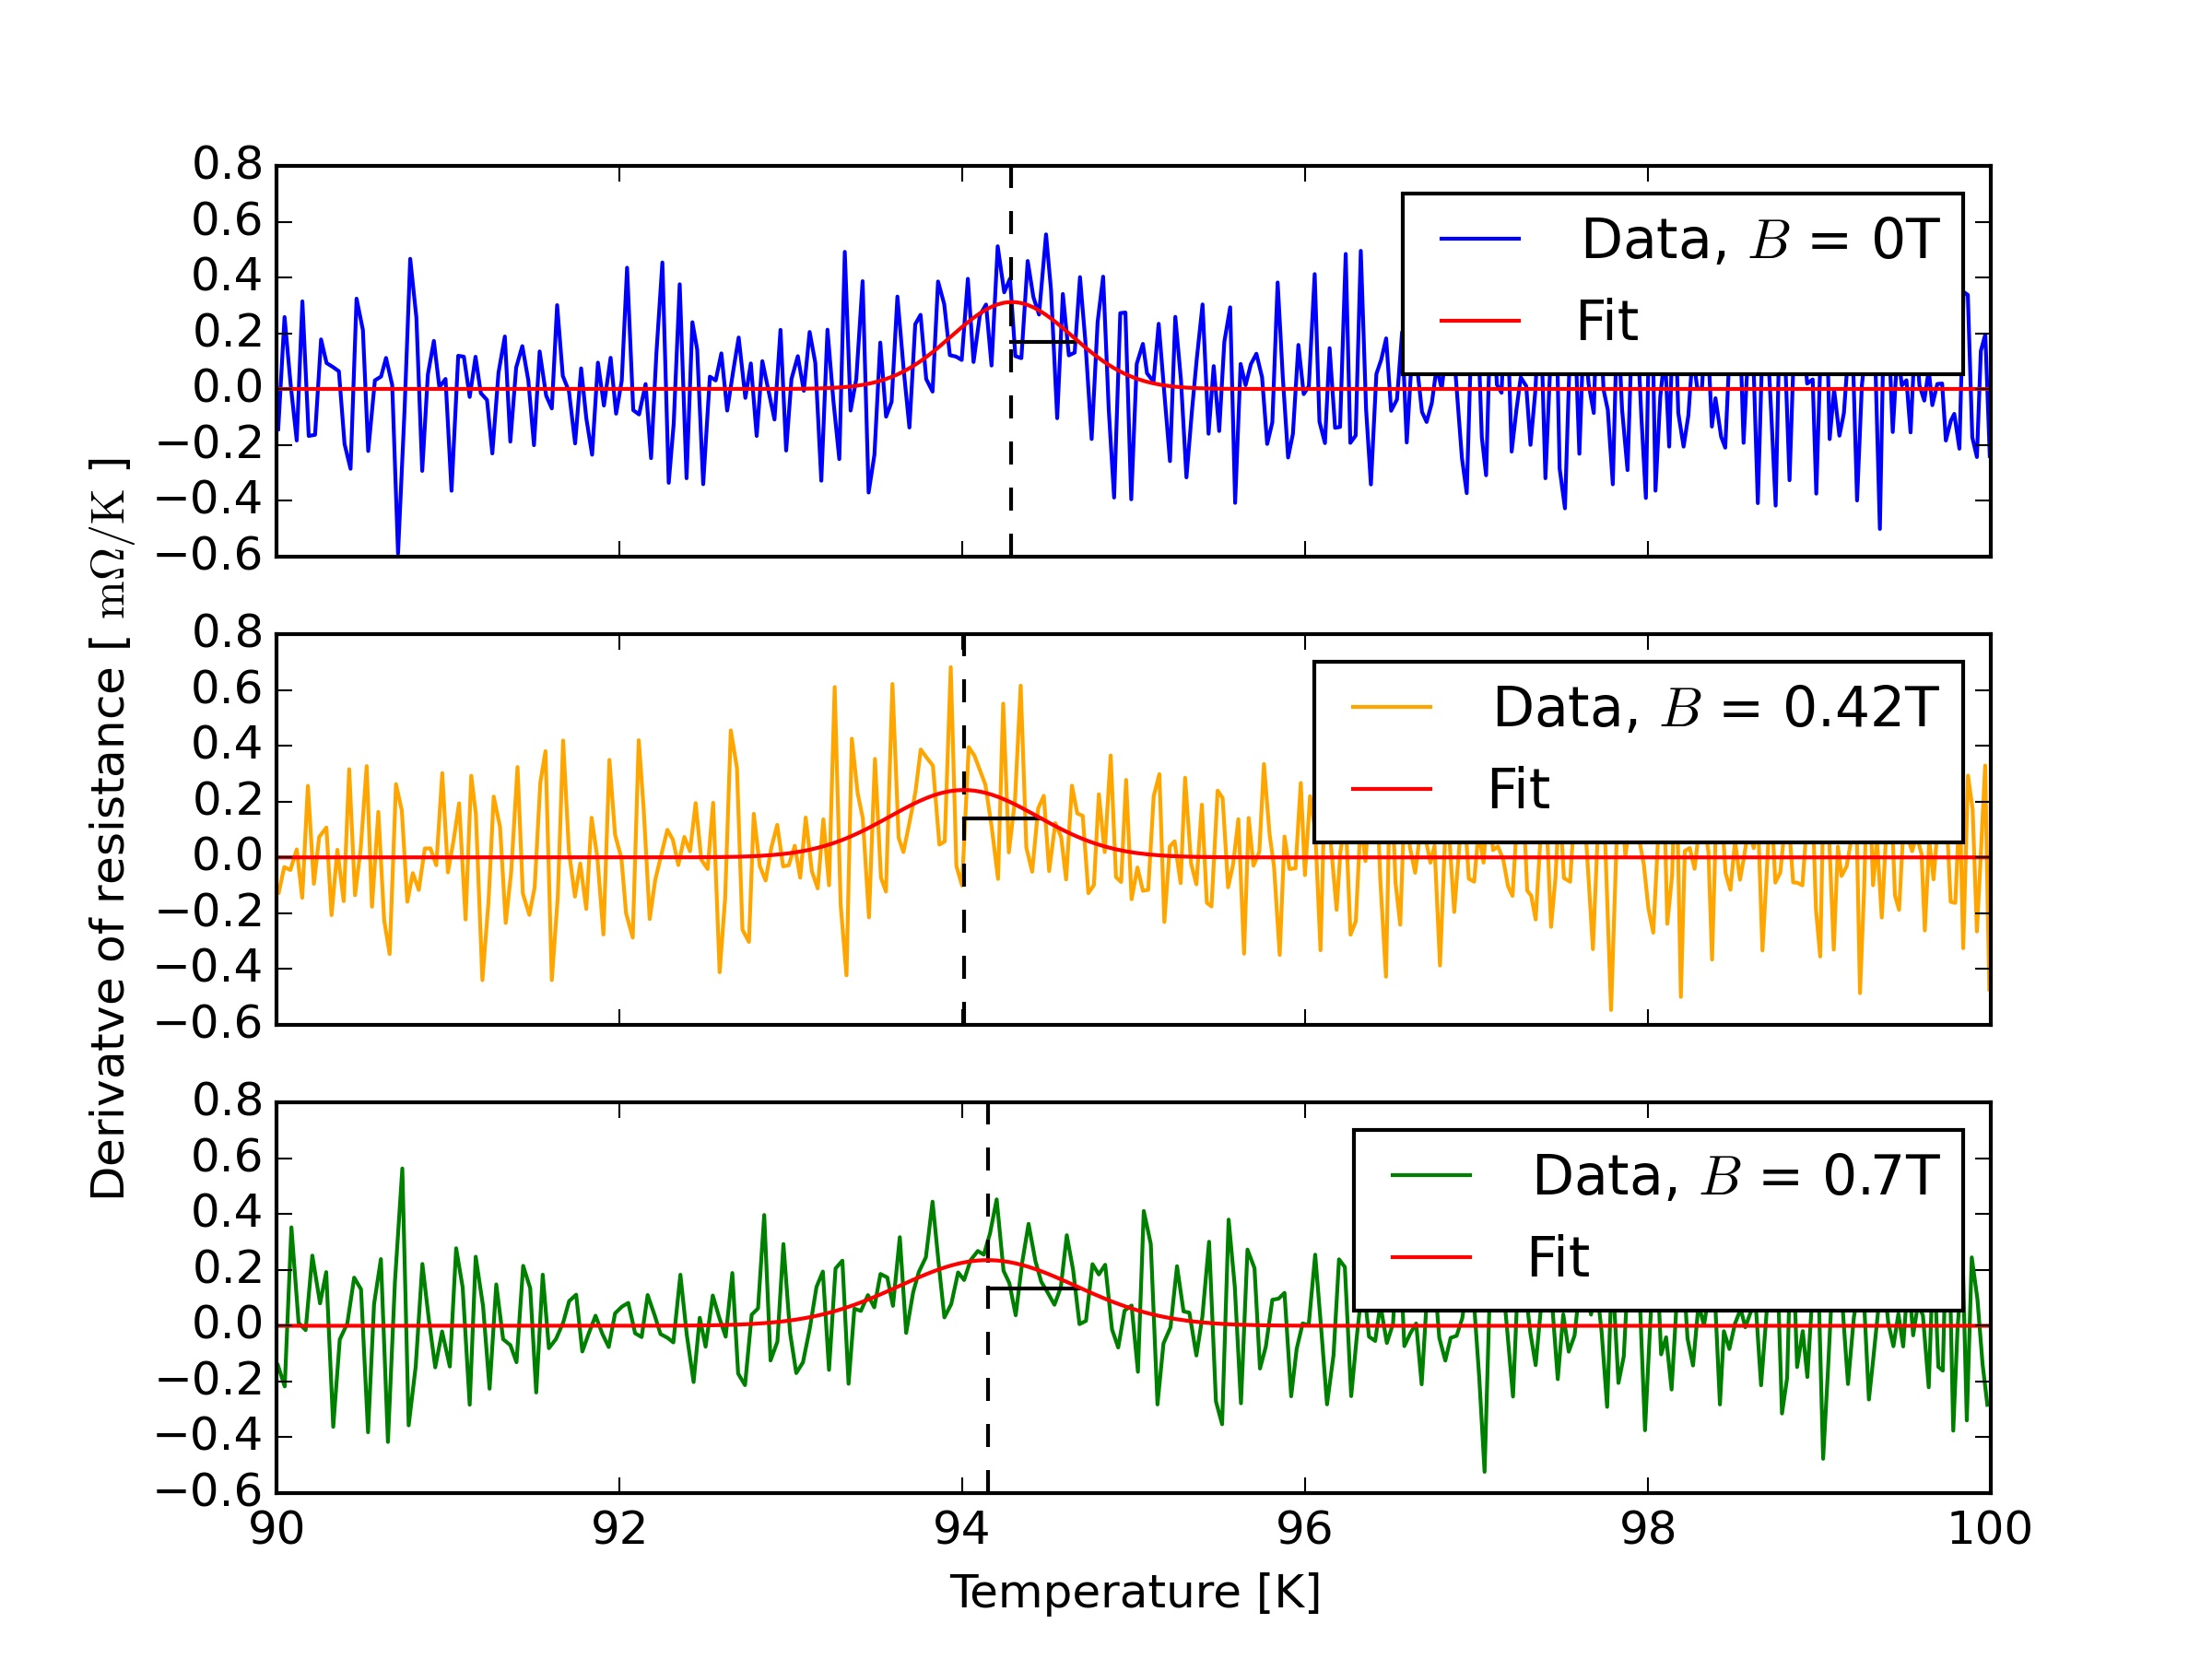
\includegraphics[scale=0.1]{Criticaltemperature3}
\caption[]{Derivative calculated the direct neighbours (h=1).  }
\label{h1}
\end{figure}
\begin{figure}[H]
\centering
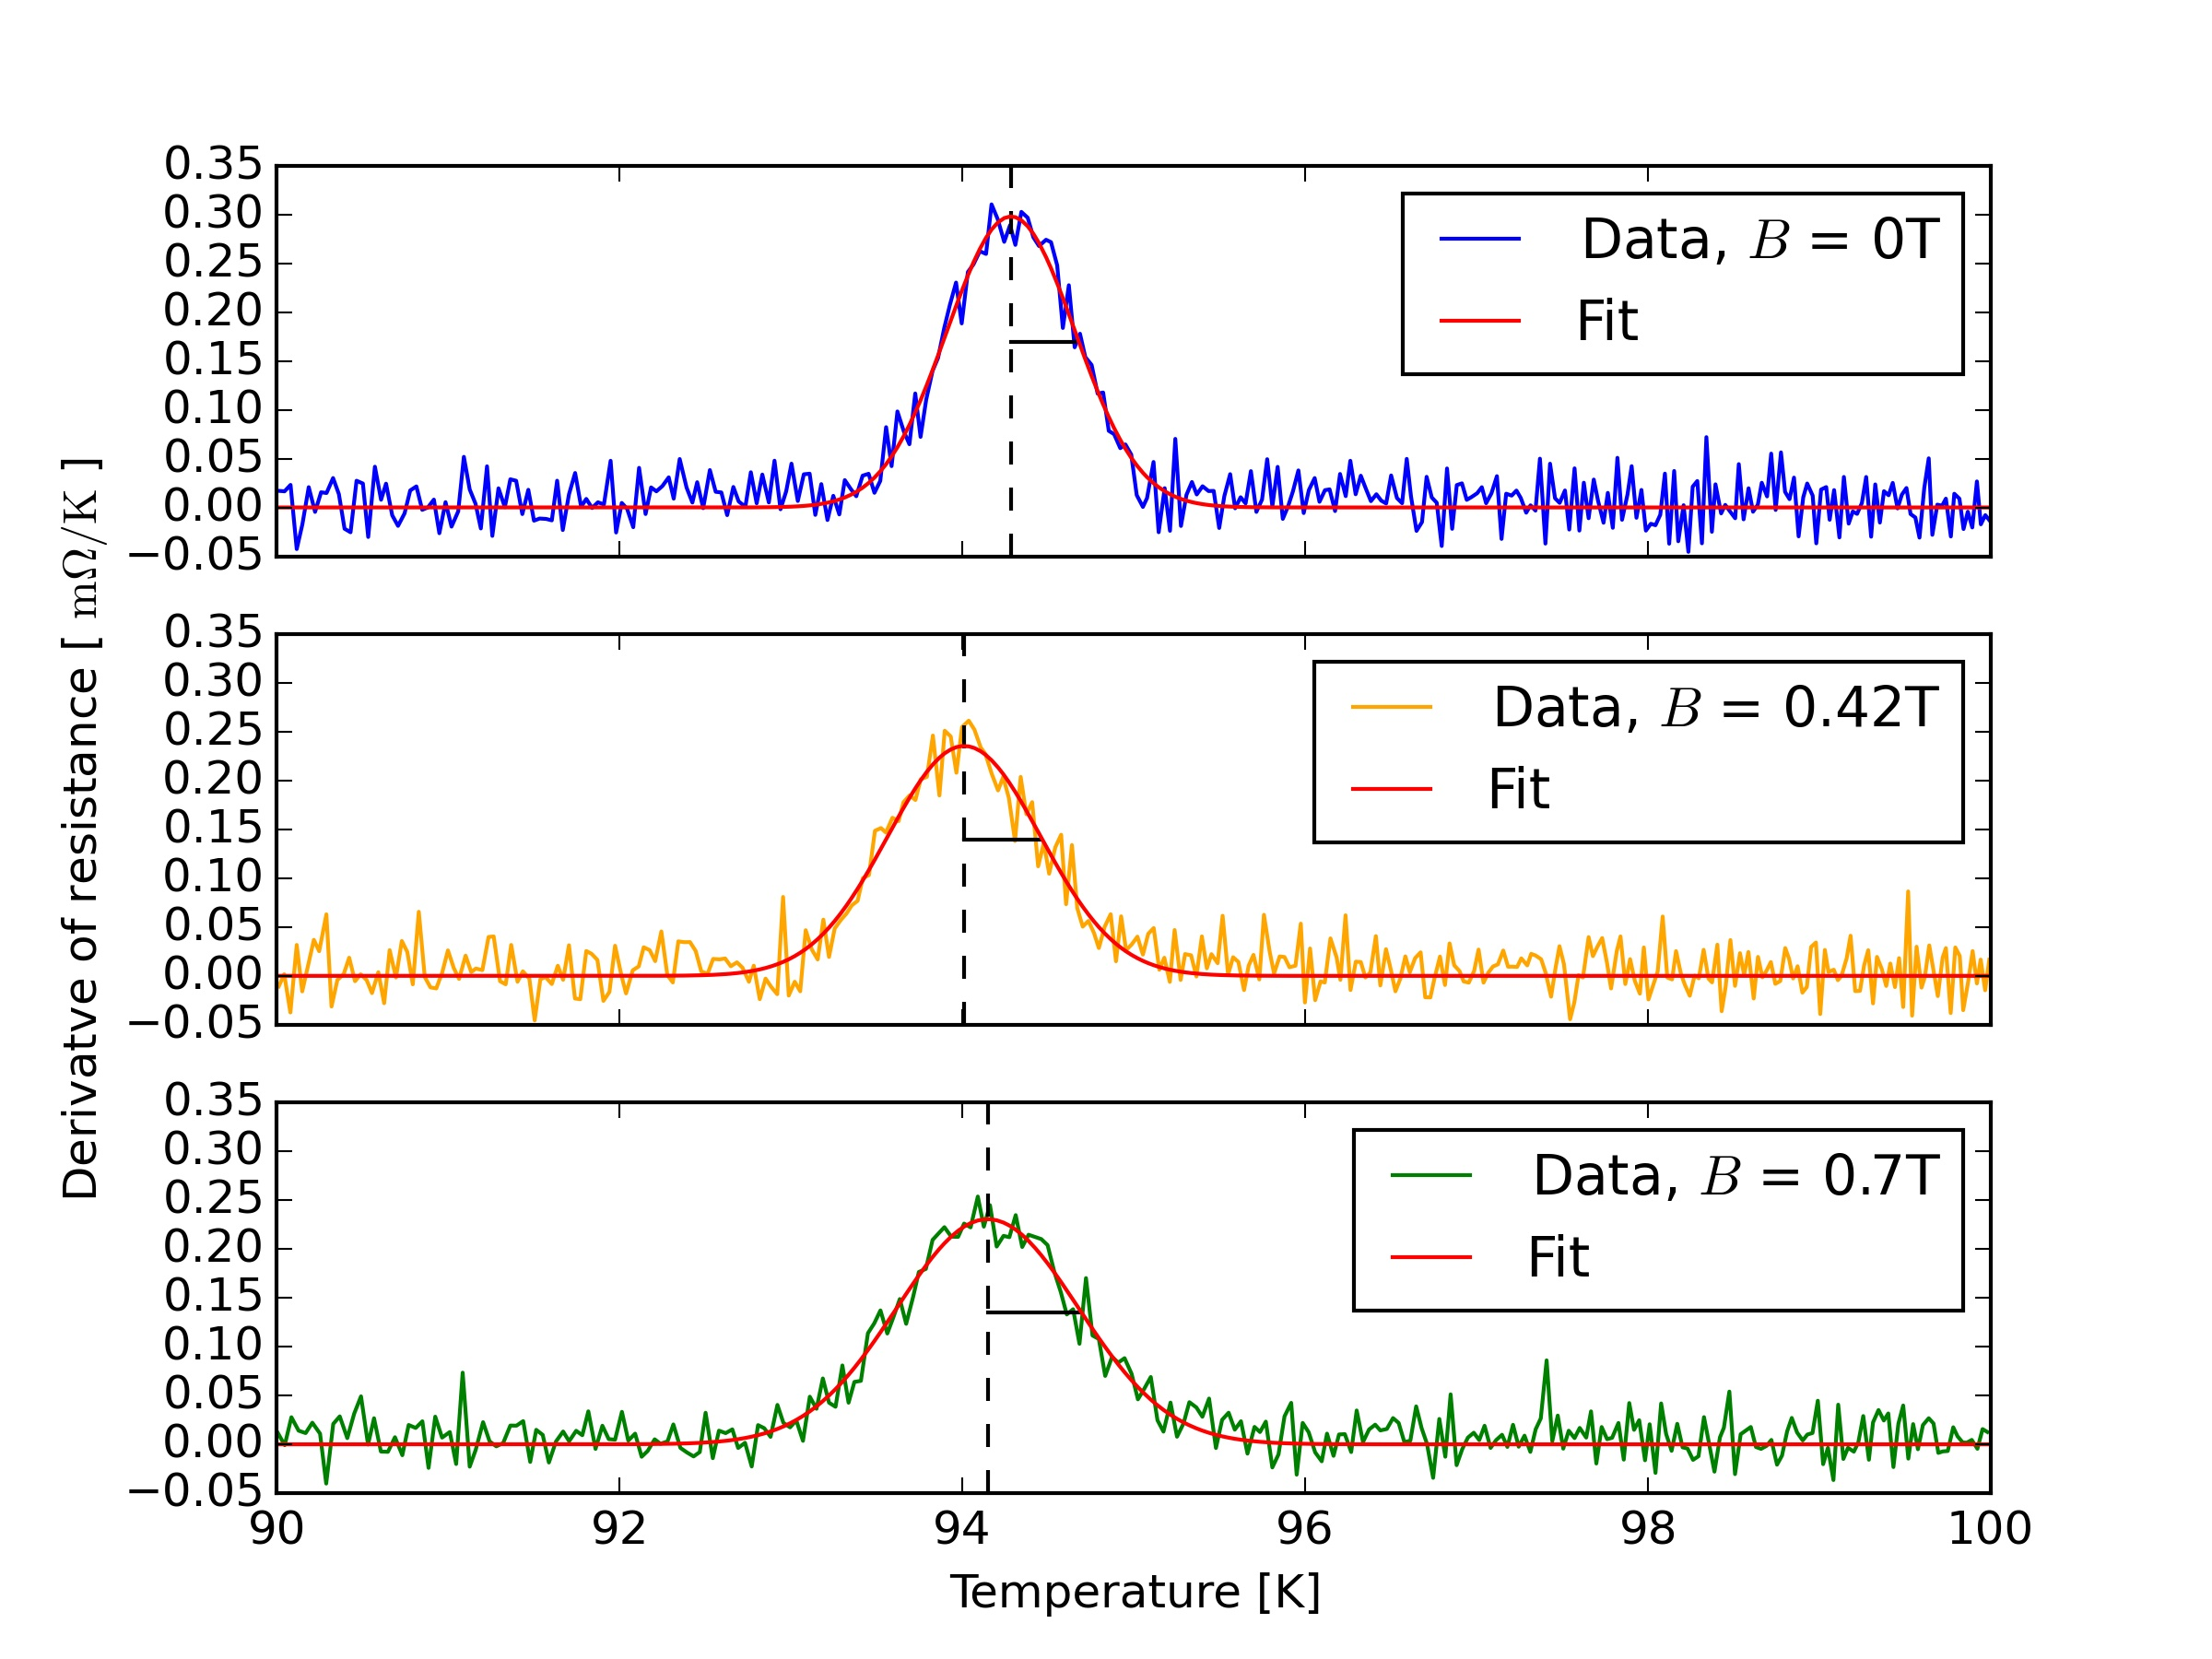
\includegraphics[scale=0.1]{Criticaltemperature2}
\caption[]{Derivative calculated with h=10.}
\label{meanresist}
\end{figure}

Fitting this data with a Gaussian distribution, and looking at its peak gives the values for the transition temperatures summed up in table \ref{results} below.


\begin{table}[H]
\centering
\renewcommand{\arraystretch}{1.2} % Abstandzwischen Zeilen
\setlength{\tabcolsep}{3mm} % Abstandzwischen Spalten
\footnotesize
\begin{tabular}{r|ccc}
$B[T]$ & 0 & 0.42 $\pm$ 0.01 & 0.70 $\pm$ 0.01 \\ 
\hline 
$T_{c} [K]$ & 94.3 $\pm$ 0.4 & 94.0 $\pm$ 0.4 & 94.1 $\pm$ 0.5 \\ 
\end{tabular}
\caption[]{Results}
\label{results}
\end{table} 
 


\item Why is the resistance measurement carried out twice with a reversion of the polarity?\\
\\
The reason behind this procedure are the contact potentials (also known as \emph{Volta potential}) of the plugs. Due to the different Fermi-energies in the different metals, in the region near the connection, some electrons move from the material with higher Fermi-energy to the other one. Thus every connection between two different metals creates a potential, with a fixed direction.  This leads to a systematic error, which shifts all measured voltages (positive and negative) to the same direction. So the voltage was measured, and the resistance calculated in both directions. Finally the mean value of the two resistances was taken to reduce the systematic error. The result of this procedure can be seen in figure \ref{widerstand07T}.
\begin{figure}[H]
\centering
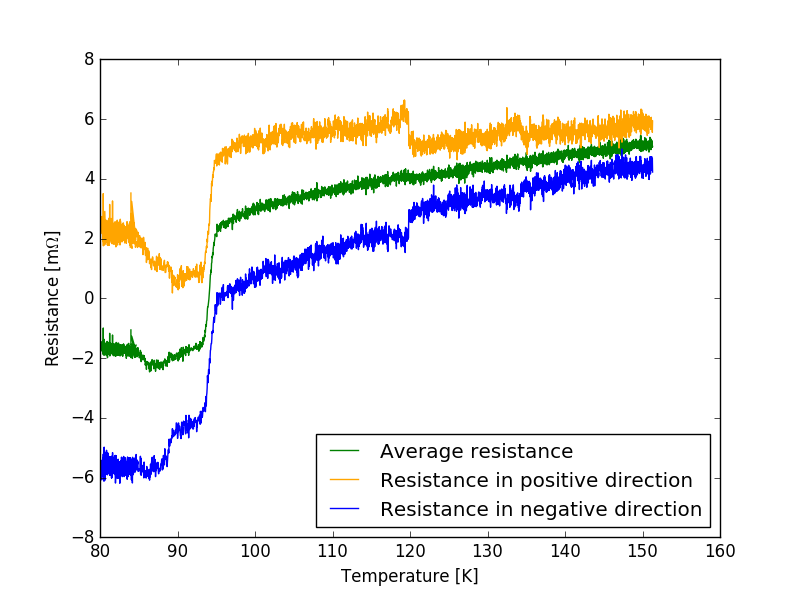
\includegraphics[scale=0.45]{widerstand07T}
\caption[]{Resistances in different directions at 0.7T}
\label{widerstand07T}
\end{figure}

\end{enumerate}

\chapter{Error calculus}

\section{Transition temperature}

Since the measurement more or less looks like a step-function one can get the error of $T_{c}$ by looking at the width of the derivative-curve. In an ideal case the derivative of a step-function would give a $\delta$-function which is localised in one point. In our case the data was fitted with a non normalized Gaussian distribution:
\begin{align*}
f(x)= a \cdot e^{\frac{1}{2} \cdot \frac{(x-\mu)^2}{\sigma^2}}
\end{align*} 
The error (width of the peak), is then directly given by the parameter $\sigma$. It is also drawn in figure \ref{meanresist}.

\chapter{Discussion}
The measured resistance curves look quite reasonable, especially for temperatures above $T_c$. Nevertheless there are some unexpected parts in the curves:
\begin{itemize}
\item Transition temperature $T_c$: \\
The literature value of the transition temperature is $92 \mathrm{K}$. This is quite near to the measured value of $(94.3 \pm 0.4) \mathrm{K}$, but it is not in the error range. There could be different reasons for this. Maybe the measured temperature was a little bit off the real temperature inside the probe. \\
Another unexpected observation is, that the transition temperature goes down if a magnetic field of $0.42 \mathrm{T}$ is applied, but goes up again a little bit if the magnetic field is raised to $0.7 \mathrm{T}$. The expectation was that $T_c$ would become lower, the larger the magnetic field is. \\
\item Below transition temperature: \\
Below $T_c$ in theory the resistance should drop to zero. In our measurements the resistance goes even down to values below zero, which makes no sense. But since it is very hard to measure such small resistances that precisely, and it is even impossible to measure zero resistance, it is not unexpected, that some errors appear in this region. 



\end{document}
